\chapter{Propuesta}\label{chapter:proposal}
En esta sección se abordan los problemas principales presentados y la solución encontrada, para cada uno, en las respectivas secciones y se profundiza sobre nuevos problemas hallados, los cuales fueron resueltos para un mejor efecto final. Por otra parte, se proponen formas de facilitar la utilización e inter-operabilidad de la propuesta presentada. 

%%%%%%%%%%%%%%%%%%%%%%%%%%%%
% MOSTRAR FOTO DE CADA PROBLEMA
%%%%%%%%%%%%%%%%%%%%%%%%%%%%

\begin{figure}[ht!]
\centering
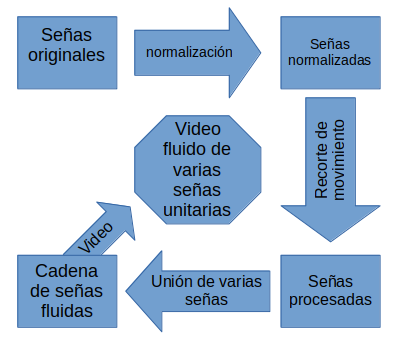
\includegraphics[width=0.5\textwidth]{./Graphics/esquema}
\caption{Esquema del enfoque a utilizar}
\label{f:enfoque_esquema}
\end{figure}

Se utilizara un enfoque basado en la interpolación de movimiento para lograr la correcta concatenación y fluidez para la generación gráfica de señas. Dado un conjunto de señas unitarias se deberá efectuar un correcto procesamiento de las mismas y lograr unir varias de ellas en un video de manera fluida, haciendo así posible la generación de señas [véase Fig \ref{f:enfoque_esquema}]. 



\section{Definiciones}

Se define como un video $V$ a la secuencia de puntos extraídos. $V_i$
constituye el i-ésimo cuadro (\emph{frame}) del video. Un frame $F$ está compuesto por una secuencia
de puntos en el espacio, representando las posiciones de las diferentes partes del cuerpo extraídas,
$F_i$ representa el i-ésimo punto del frame y $F_{parte}$ representa los puntos asociados a la parte 
descrita en el frame. 

\subsection{Operaciones vectoriales}

Las operaciones vectoriales constituye operaciones realizadas sobre los vectores. Estas operaciones 
pueden representar diferentes acciones a un nivel de abstracción mayor sobre los vectores. Sean $a$ y
$b$ vectores o puntos de tres dimensiones entonces:

\begin{itemize}
	\item $a - b$: Representa el vector de la dirección del punto $b$ hacia $a$.
	\item $a + b$: Representa la traslación del punto $a$ ($b$) en dirección $b$ ($a$).
	\item $a \times b$: Representa un vector perpendicular a $a$ y $b$.
	\item $\cos \theta = \frac{a \cdot b}{||a|| \cdot ||b||}$: Representa el coseno del ángulo $\theta$
	entre los vectores $a$ y $b$.
	\item $\alpha a$: Representa el vector siendo escalado por un factor $\alpha$.
\end{itemize}

\subsubsection{Rotación de Rodríguez}

La rotación constituye en girar sobre un eje $k$ un vector $v$, $\theta$ grados, donde ambos vectores son 
unitarios. Este vector rotado puede ser hallado mediante:
$$
rotación(v, k, \theta) = v \cos \theta + (k \times v) \sin \theta + k(k \cdot v)(1 - \cos \theta)
$$.


\section{Preprocesamiento de los datos}
Al utilizar datos por primera vez siempre es una buena práctica analizarlos y reconocer la estructura que poseen. La gran mayoría de las veces los datos con los que se trabaja vienen originalmente con fallas estructurales o de valores que no pertenecen al dominio que se trabaja. Es por este motivo que se hace fundamental, siempre que se vaya a realizar un trabajo con datos, realizarle su correspondiente análisis estructural y detectar posibles errores que se contengan en los mismos.
\subsection{Obteniendo el conjunto de datos}
De anteriores investigaciones contamos con un corpus de señas unitarias las cuales tienen la siguiente estructura :
$$
(r,f,p,c)
$$
 
donde :
\begin{itemize}
 \item $r$ indica la representación a la que se accede de dicha frase nominal en el conjunto de datos.
 \item $f$ refiere al frame al que se accede de dicha representación
 \item $p$ representa el punto al que se indexa de dicho frame
 \item $c$ indica la componente del punto a la que se accede
\end{itemize}
 
  Una seña unitaria no es más que una secuencia que representa a una frase nominal, dígase como ejemplo la seña que significa  ``américa del sur''. 

\subsection{Limitando a una sola seña por frase}
Luego de tener el conjunto de frases curadas y limpias, quedaba aún el problema de las palabras repetidas que tienen más de una seña, en dependencia de qué léxico del corpus brindado por el CENDSOR se revise.
Para dicho problema se optó por escoger solamente la primera que apareciera, puesto que solo complejizaría más la tarea presentada dado que, para una misma frase en el corpus, podía incurrir en una variación bastante considerable, es decir, la señas para una misma palabra de un intérprete a otro variaban mucho para el caso de la palabra ``paz'' con 4 tipos de señas distintas (como si de una ``falta de ortografía'' se tratase). 

\subsection{Detección de problemas}
A pesar de que todos los videos poseen una estructura similar, manteniéndose un fondo fijo de un color constante, los señantes presentes en los mismos son distintos unos de otros, así como también sus movimientos realizados. Aun refiriéndose a la misma seña, las diferencias no dejaban de aparecer, tanto en estructura corporal, como en velocidad y variaciones de la seña.

En algunos casos, los videos presentaban una secuencia de imágenes sin señante inicialmente, lo que generaba que el modelo dedicado al reconocimiento corporal fallara en dicha tarea, devolviendo un conjunto de ceros, en esos cuadros (frames). Algo similar, ocurría cuando no se detectaban bien las manos del intérprete (ya sea por salirse de la ventana de enfoque de la cámara o encontrarse de forma perpendicular a la misma), haciendo que estas no aparezcan en algún que otro frame.

Para el primer caso la solución fue, sencillamente, no tomar en cuenta los frames que todos sus puntos fueran nulos; mientras que el segundo caso no era tan trivial puesto que, a pesar de no tener las manos, el cuerpo si se detecta y proporciona información importante del movimiento del señante por lo que se decidió dejar dichos conjuntos para una posterior revisión.

\subsubsection{Análisis preliminar de los datos}

Al analizar los datos se encontraron varios problemas:
\begin{itemize}
	\item Los puntos asociados a las manos no se encontraban sobre las muñecas.
	\item Los puntos de las manos no existían en intervalos del video.
	\item El tamaño del señante varía entre videos.
	\item El video contiene frames en los cuales no se realiza ningún movimiento.
\end{itemize}

\subsection{Limpieza de los datos}

 A todas las palabras se le hace limpieza con expresiones regulares para eliminar la mayoría de imperfecciones posibles en las palabras, el uso de ``nn'' en lugar de la ``ñ '' y la presencia de números puesto que al agrupar las frases de varios léxicos distintos, estos se renombraban. Este procesamiento de las palabras es de utilidad para conformar el dataset lo más preciso posible, evitando la repetición de las frases.
 
\subsubsection{Arreglando errores ortográficos}

Durante la creación del conjunto de datos se detectaron, además, frases nominales inexistentes y/o con errores ortográficos, corrigiéndose una pequeña cantidad de estas a mano con un diccionario de palabras, dado que la gran mayoría de los errores ortográficos eran tildes ausentadas.

\section{Problema de la visualización de los datos}
Los datos ya procesados, del trabajo de Gutiérrez-González \brackcite{leynier-lsc-2021}, son solamente arreglos de dimensión (número de interpretaciones de la seña, (número de frames de la seña,  número total de puntos * 3)), lo cual no facilita  interpretar o detectar posibles problemas. Para solventarlo se recurrió a graficar los puntos en un espacio tridimensional. Se realizaron las transformaciones pertinentes (rotación por el eje z y usando un grado de elevación de 90 grados)  para que se visualizara de frente al espectador, permitiendo, al tener guardada información de las uniones, la visualización de líneas entre dichos puntos espaciales.

\begin{figure}[ht!]
    \centering
    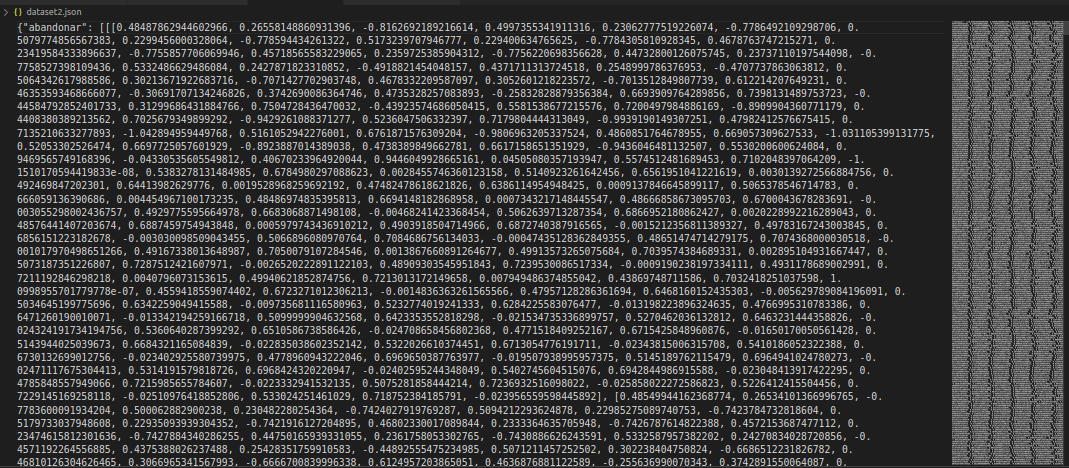
\includegraphics[width=0.6\textwidth]{Graphics/data_example.png}
    \caption{Ejemplo parcial de la representación de los datos dentro de uno de los conjuntos de datos. Se puede apreciar la frase nominal ``abandonar' seguida de parte de su representación'}
    \label{fig:data_example}
\end{figure}


Se utilizan solamente los puntos del cuerpo y de las manos obtenidos a través de la investigación antes mencionada. Se constan de 67 puntos espaciales siendo 25 del cuerpo y la cabeza (obviando el tren inferior de puntos), 21 para la mano derecha e ídem para la mano izquierda [Fig \ref{fig:points}]. 

\begin{figure}[ht!]
    \centering
    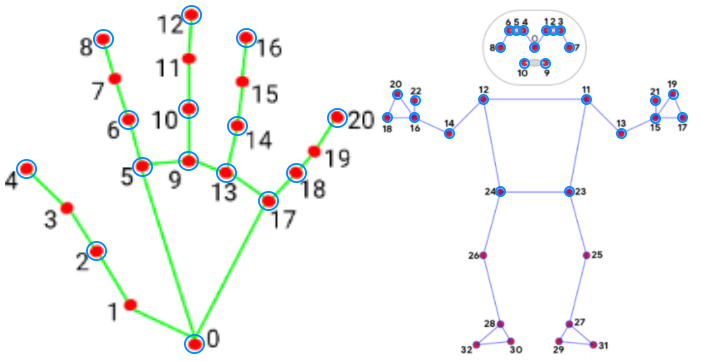
\includegraphics[width=0.6\textwidth]{Graphics/points.png}
    \caption{Algunos de los puntos que extrae Mediapipe Holistic. De izquierda a derecha apreciamos los puntos de la mano derecha y los puntos del cuerpo.}
    \label{fig:points}
\end{figure}

\section{Problema de manos que no se encontraban sobre las muñecas}

Las manos en los datos se encuentran definidas como una secuencia de puntos $F_{mano\_izquierda}$ y 
$F_{mano\_derecha}$, en ambos casos el primer punto de cada una representa el punto asociado a la muñeca 
en la mano. A su vez el cuerpo posee otra representación de la muñeca $F_{muñeca\_cuerpo\_izquierda}$ y $F_{muñeca\_cuerpo\_derecha}$. 
Estos puntos en los datos deberían
estar juntos o relativamente cercanos, sin embargo, en los datos se encontraban a una distancia considerable.

Para la solución del problema se calcula el vector dirección entre las representaciones de las muñecas del cuerpo 
y las muñecas de las manos y se trasladan los puntos de las manos en esta dirección, dejando ambas muñecas en el 
mismo sitio.

\begin{align}
d &= F_{muñeca\_cuerpo\_izquierda} - F_{muñeca\_mano\_izquierda} \\
F_{mano\_izquierda}' &= F_{mano\_izquierda} + d
\end{align}

\section{Problema de las manos faltantes}

Este problema consiste en que en ciertas secciones del video los puntos asociados a las manos fallan al ser 
encontrados por los modelos de reconocimiento [véase Fig \ref{f:manos_faltantes}]. Este problema se divide en dos casos:

\begin{itemize}
\item Faltan en los frames internos de la seña [véase Fig \ref{f:manos_faltantes}]
\item Faltan las manos en los frames extremos de la seña [véase Fig \ref{f:fluidez_variable}]
\end{itemize}

\begin{figure}[t]
	\begin{subfigure}[t]{0.3\textwidth}
	\centering
		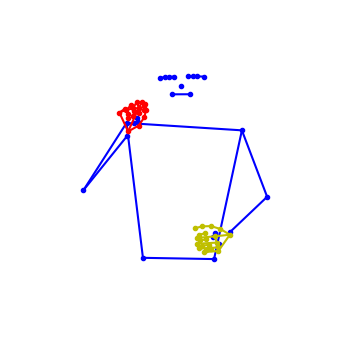
\includegraphics[align=t,width=0.9\linewidth, height =0.9\linewidth]{Graphics/mano_antes_desaparecer.png}
		\caption{Mano antes de desaparecer del token ``aborto''}
		\label{f:mano_antes_desaparecer}
	\end{subfigure}
	\begin{subfigure}[t]{0.3\textwidth}
	\centering
		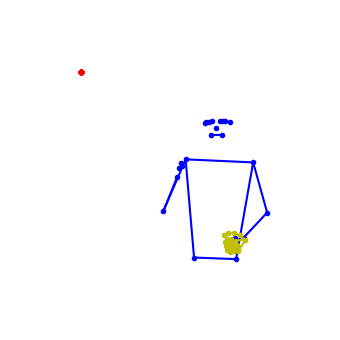
\includegraphics[align=t,width=0.9\linewidth, height =0.9\linewidth]{Graphics/mano_desaparecida.png}
		\caption{Mano derecha desaparecida del mismo token al siguiente frame }
		\label{f:mano_derecha_desaparecida}
	\end{subfigure}
		\begin{subfigure}[t]{0.3\textwidth}
	\centering
		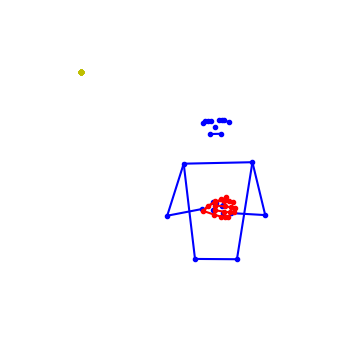
\includegraphics[align=t,width=0.9\linewidth, height =0.9\linewidth]{Graphics/mano_faltante_interna.png}
		\caption{Mano izquierda desaparecida del mismo token en otro frame distinto}
		\label{f:mano_izquierda_desaparecida}
	\end{subfigure}
	\caption{Ejemplo del segundo caso de  manos faltantes.}
	\label{f:manos_faltantes}
\end{figure}

\subsection{Frames internos}
La solución propuesta para el primer caso es interpolar las posiciones intermedias faltantes teniendo como 
partida los últimos puntos existentes de las manos antes de desaparecer y como llegada los primeros puntos existentes 
luego de la desaparición. Para esto se define el operador interpolación $I$, el cual toma dos conjuntos de puntos, los 
puntos de partida y los de llegada, y un número representando la cantidad de elementos a devolver uniformemente
escogidos en el intervalo a interpolar. El resultado de aplicar 
$I(V[i]_{mano\_izquierda}, V[i + k]_{mano\_izquierda}, k - 1)$ es el conjunto interpolado de $k-1$ frames 
entre los frames $i$ e $i+k$. Al aplicar este método en cada intervalo en los cuales no estaba definida las manos 
se llenan estos huecos.
\subsection{Frames extremos}
En el segundo caso no se puede realizar la interpolación, debido a que no existe un conjunto de llegada o de partida. Al probar con distintos conjuntos de señas, resaltó el hecho de que las señas que comenzaban sin manos, durante un largo período de tiempo, causaban errores y fallos en la solución de la sección \ref{section:proposal:fluidez}.  Por lo que la forma de resolver dicho inconveniente devino del uso de una mano falsa, como si de una prótesis se tratara, la cual se compone del mismo número de puntos de una mano real y la misma fue situada gracias a que el cuerpo contiene puntos coincidentes para este mismo propósito.

Para resolver el problema se creó una mano en posición semi-extendida para que actuara de prótesis en los lugares 
donde ocurre el problema. Esta mano prótesis necesita ser modificada para que se pueda colocar en el lugar correcto 
en cuerpo. En primer lugar se realiza una rotación de esta de tal forma que quede alineada con el brazo, luego dicha 
mano es trasladada hacia la muñeca del cuerpo.

Se realizaron transformaciones espaciales, rotaciones y se seleccionaron matrices específicas para operar con los puntos de la mano falsa y así obtener su homologa contraria, además de permitir ajustarla al plano regido por el codo, la muñeca y los tres puntos coincidentes. Todo este conjunto de operaciones, sumado al hecho de utilizar la proporción de cuanto mide el antebrazo respecto a la medida desde la muñeca y la base del dedo medio, permitieron el correcto estiramiento y adaptación de la mano falsa a las distintas estructuras corporales evidenciadas en el conjunto de datos.

\begin{align}
\begin{split}
brazo\_izq &= normalizar(F_{muñeca\_cuerpo\_izquierdo} - ... \\
& F_{codo\_izquierdo})
\end{split}\\
\begin{split}
muñeca\_izq\_dirección &= normalizar(F_{muñeca\_mano\_izquierda} - ... \\
& F_{nudillo\_dedo\_medio\_izquierdo})
\end{split}\\
eje\_rotación &= normalizar(brazo_izq \times muñeca\_izq\_dirección) \\
ángulo &= \arccos brazo\_izq \cdot muñeca\_izq\_dirección \\
F_{mano\_izquierda} &= rotación(F_{mano\_izquierda}, eje\_rotación, ángulo) \\
d &= F_{muñeca\_cuerpo\_izquierda} - F_{muñeca\_mano\_izquierda} \\
F_{mano\_izquierda} &= F_{mano\_izquierda} + d
\end{align}

\section{Problema de la fluidez en la unión de varias señas}\label{section:proposal:fluidez}
La fluidez en la generación de avatares es de vital importancia, puesto que una de las metas es lograr la mayor semejanza posible al movimiento natural de una persona. Al pensar en concatenar dos señas lo primero que se imagina es un movimiento suave y que se logren identificar ambas secuencias, cosa que no ocurre al unir dos secuencias sin ningún tipo de procesamiento como los videos con que se cuentan. No todos los intérpretes terminaban la seña de la misma manera, ni en la misma posición [véase Fig \ref{f:fluidez_variable}], y en algunos casos hasta ocurrían periodos largos de inactividad entre que terminaba la seña y el final del grabación. 


La solución encontrada a este problema fue interpolar entre ambas secuencias, obtando por la interpolación cúbica como candidata de mayor suavidad, si se requieren bastantes frames intermedios, y la lineal para casos de pocos frames o poca variación de movimiento.
Esta interpolación se realiza escogiendo una cantidad fija de puntos en dependencia del método escogido. Dichos puntos son separados por componentes y  se realiza la interpolación de forma individual en función de una lista de valores ``t'' asociados a cada una. Es decir, una lista t que enumera los valores de x es el argumento de la función a interpolar, dejándose por medio los valores asociados a la cantidad a interpolar, mientras que los valores obtenidos en la lista x serían los valores de la evaluación de dicha función en los valores de t conocidos.

\subsection{Frames variables intermedios}
Durante la concatenación también existe un diferencial de movimiento entre el final de una seña y el inicio de otra. El problema aquí es 
que existen poses que terminan más distantes de su continuación que otras, haciendo que 
la transición sea o muy rápida o muy lenta, por esto se decide hacer una transición con frames
variables en dependencia de la diferencia. Algunos de los videos terminan reposando ambas manos superpuestas sobre el vientre, mientras que en otros se termina descansando los brazos paralelamente al cuerpo o terminan de cualquier otra forma. Además, la distancia del señante a la cámara es, también, muy variable, por lo que se denota como movimiento dada la diferencia de posición.

\subsection{Unión de señas}

La unión de señas constituye la operación de unir dos señas para conformar una sola. Esta operación
es realizada mediante el operador de interpolación al unir los videos $V_1$ y $V_2$, una vez realizadas todas 
las operaciones anteriores, de la siguiente forma:

\begin{equation}
V = I(V_1[n], V_2[0], frames\_de\_intercambio)
\end{equation}

Se observa que hace falta conocer la cantidad de $frames\_de\_intercambio$, este valor debe depender de la diferencia
entre $V_1[n]$ y $V_2[0]$ ya que vectores parecidos deben de tener menos frames de transición que vectores más distantes [véase Fig \ref{f:fluidez_variable}).
Se define diferencia como la norma de la diferencia entre los vectores.

A criterio del autor se seleccionaron unos ejemplos en donde se sabía la variabilidad y la cantidad de frames buenas para el segmento a interpolar. Para obtener este valor se observaron varios valores de diferencia entre vectores y se decidió la cantidad de frames de 
intercambio para dicha diferencia [véase Tabla \ref{table:intercambio_frame}], con varias muestras se creó una función mediante interpolación de estos valores la cual 
permite conocer el valor de $frames\_de\_intercambio$ dada la diferencia.


\begin{table}[h!]
	\begin{center}
	  \caption{Valores a criterio del autor para interpolar según la variación de movimiento entre frames }
	  \label{table:intercambio_frame}
	  \begin{tabular}{c|c} 
		\textbf{Variación entre frames} & \textbf{Cantidad de frames}\\
		\hline
		0.0 & 1 \\
		0.5 & 7 \\
		4.6 & 14\\
	  \end{tabular}
	\end{center}
  \end{table}

\begin{figure}[t]
\centering
	\begin{subfigure}[t]{0.3\textwidth}
		\centering
		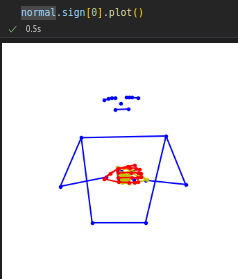
\includegraphics[align=t,width=0.9\linewidth, height =0.9\linewidth]{Graphics/principio_abandonar.png}
		\caption{Principio del token ``abandonar''}
		\label{f:principio_variable_abandonar}
	\end{subfigure}
		\begin{subfigure}[t]{0.3\textwidth}
		\centering
		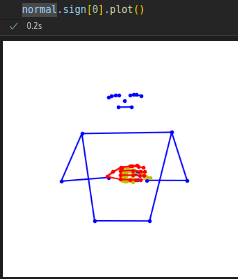
\includegraphics[align=t,width=0.9\linewidth, height =0.9\linewidth]{Graphics/principio_aborto.png}
		\caption{Principio del token ``aborto''}
		\label{f:principio_variable_aborto}
	\end{subfigure}
		\begin{subfigure}[t]{0.3\textwidth}
		\centering
		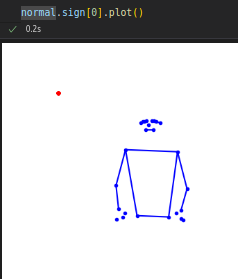
\includegraphics[align=t,width=0.9\linewidth, height =0.9\linewidth]{Graphics/principio_amar.png}
		\caption{Principio del token ``amar''}
		\label{f:principio_variable_amar}
	\end{subfigure}	
	\vskip 0pt
	\begin{subfigure}[t]{0.3\textwidth}
		\centering
		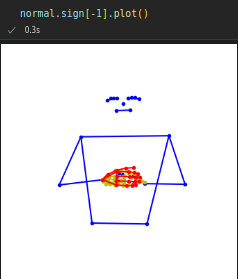
\includegraphics[align=t,width=0.9\linewidth, height =0.9\linewidth]{Graphics/final_abandonar.png}
		\caption{Final del token ``abandonar''}
		\label{f:final_variable_abandonar}
	\end{subfigure}
	\begin{subfigure}[t]{0.3\textwidth}
		\centering
		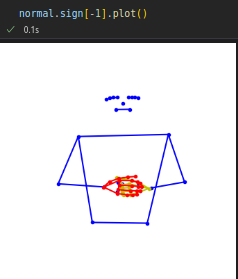
\includegraphics[align=t,width=0.9\linewidth, height =0.9\linewidth]{Graphics/final_aborto.png}
		\caption{Final del token ``aborto''}
		\label{f:final_variable_aborto}
	\end{subfigure}
	\begin{subfigure}[t]{0.3\textwidth}
		\centering
		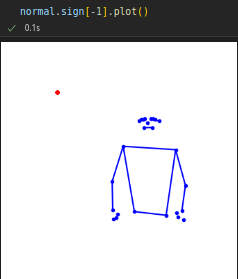
\includegraphics[align=t,width=0.9\linewidth, height =0.9\linewidth]{Graphics/final_amar.png}
		\caption{Final del token ``amar''}
		\label{f:final_variable_amar}
	\end{subfigure}
	
	\caption{Ejemplo de la diferencia entre extremos consecutivos de varios tokens, evidenciándose su variabilidad.}
	\label{f:fluidez_variable}
\end{figure}
El hecho de usar uno u otro método de interpolación, implica que se seleccionan distintas cantidades de puntos, como se explica en el estado del arte [véase sección \ref{section:state-of-the-art:interpolation}] . Siendo la más dinámica, con una menor cantidad de puntos, la interpolación lineal, pero, mínimo, se cuenta con 24 frames ya que equivalen a 1 segundo de un video de 24 fps(frames por segundo), lo cual es bastante estándar.


\subsection{Problema del tamaño del señante variable durante el video}

En los videos analizados se encuentran varios tipos de señante, estos tienen diferentes complexiones y también
se encuentran grabados desde diferentes distancias e inclinaciones. Esto trae como consecuencia que los puntos 
extraídos no tengan la misma configuración. Para esto se normalizan los puntos de cada frame $F$ teniendo como 
referencia la distancia entre los hombros. Esta distancia en cada frame es mantenido constante a un valor de $0.5$. Para lograr esto 
primero se calcula el factor de escalado del frame para que la distancia entre los hombros sea $0.5$ y luego este 
factor es aplicado a todos los puntos, logrando así una mayor homogeneidad entre los distintos señantes.

\begin{align}
factor\_de\_normalización &= \frac{0.5}{|| F_{hombro\_derecho} - F_{hombro\_izquierdo} ||} \\
F &= factor\_de\_normalización \cdot F
\end{align}

Con estas operaciones se mantiene una distancia constante de $0.5$ en cada frame.


\subsection{Inactividad en la secuencia}
Este problema surge debido a la naturaleza de los videos analizados. En estos el señante empieza y termina en una 
posición de descanso por lo que en esta etapa no ocurre un movimiento relativo a la seña descrita. Esto implica 
que al realizar la concatenación de videos aparecieran periodos con estas posiciones de descanso, lo cual impedía
una concatenación fluida. Esto no conlleva una solución tan trivial como simplemente recortar los frames con una cantidad fija, dado que cada video puede presentar anomalías que lo hagan parecer inactivo o pueden existir videos sin inactividad, con lo cual, al recortar, estaríamos eliminando parcialmente la seña. Para la solución de dicho problema se define una ecuación que mide el movimiento
en el video, luego nos quedamos con el intervalo de video que contenga la mayor parte del movimiento 
total del mismo y que tenga un intervalo lo más pequeño posible.

La ecuación de movimiento se define como:

\begin{equation}
mov(i) = || V[i+1] - V[i] ||
\end{equation}

Esta ecuación cuantifica el movimiento entre un frame y el próximo y por su definición es no negativa [véase Fig \ref{f:movediff_aborto_amar}], 
por lo tanto hallando su integral en el dominio se puede tener una medida del movimiento en el segmento.
Se defina la integral de $mov$ en el intervalo $i$, $j$ como:

\begin{equation}
integral\_mov(i,j)
\end{equation}

Se desea obtener un intervalo que contenga gran parte del movimiento pero que no sea el video completo, para esto 
se define el problema de optimización siguiente, donde $n$ es el frame final:

\begin{align}
\max_{i,j} &\frac{integral\_mov(i,j)}{j-i} \\
s.a: \qquad integral\_mov(i,j) &> integral\_mov(0,n) \cdot porciento\_de\_movimiento \\
& \qquad j > i
\end{align}

Obteniendo el intervalo que solucione el problema anterior se obtiene un nuevo video al quedarse solamente con los 
frames dentro de este intervalo, que aseguran que el movimiento en este es mayor al $porciento\_de\_movimiento$ seleccionado.
Dado que el problema es discreto la integral es calculada por métodos numéricos y el problema de optimización es 
resuelto probando los valores posibles de los intervalos $i,j$.

\begin{figure}[t]
	\begin{subfigure}[t]{0.3\textwidth}
	\centering
		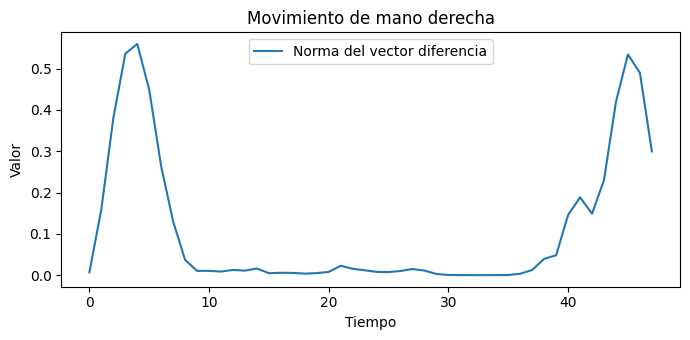
\includegraphics[align=t,width=0.9\linewidth, height =0.9\linewidth]{Graphics/amar_rhand_movediff_original_nu.png}
		\caption{Gráfica de movimiento de la mano derecha del token ``amar''}
		\label{f:rhand_movediff_amar}
	\end{subfigure}
	\begin{subfigure}[t]{0.3\textwidth}
	\centering
		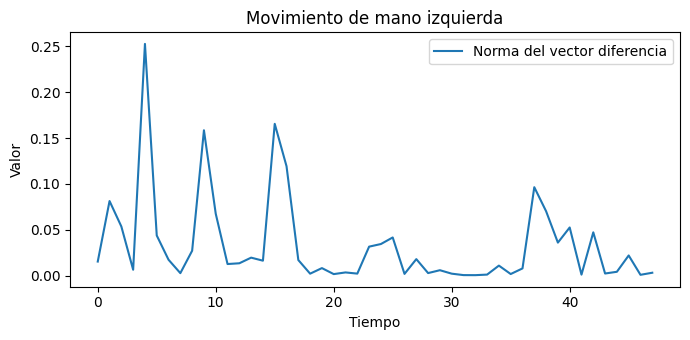
\includegraphics[align=t,width=0.9\linewidth, height =0.9\linewidth]{Graphics/amar_lhand_movediff_original_nu.png}
		\caption{Gráfica de movimiento de la mano izquierda del token ``amar'' }
		\label{f:lhand_movediff_amar}
	\end{subfigure}
		\begin{subfigure}[t]{0.3\textwidth}
	\centering
		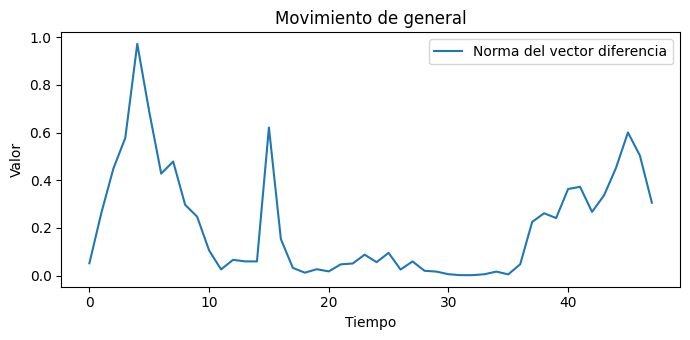
\includegraphics[align=t,width=0.9\linewidth, height =0.9\linewidth]{Graphics/amar_global_movediff_original_nu.png}
		\caption{Gráfica de movimiento general del token ``amar''}
		\label{f:general_movediff_amar}
	\end{subfigure}
	\vskip 0pt
	\begin{subfigure}[t]{0.3\textwidth}
	\centering
		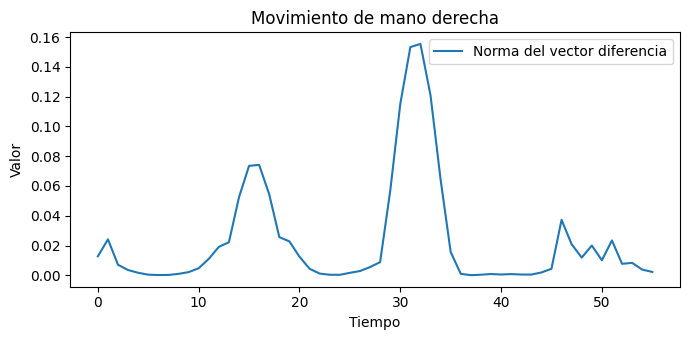
\includegraphics[align=t,width=0.9\linewidth, height =0.9\linewidth]{Graphics/aborto_rhand_movediff_original_nu.png}
		\caption{Gráfica de movimiento de la mano derecha del token ``aborto''}
		\label{f:rhand_movediff_aborto}
	\end{subfigure}
	\begin{subfigure}[t]{0.3\textwidth}
	\centering
		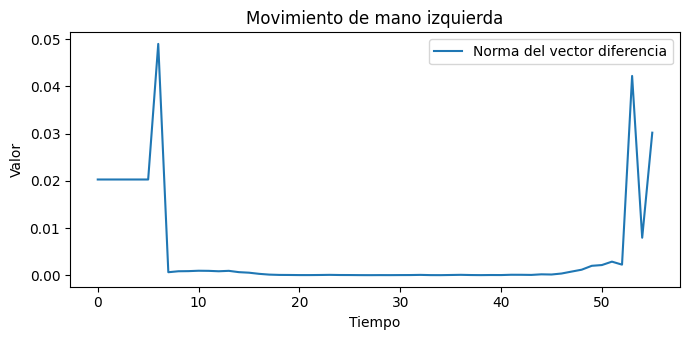
\includegraphics[align=t,width=0.9\linewidth, height=0.9\linewidth]{Graphics/aborto_lhand_movediff_original_nu.png}
		\caption{Gráfica de movimiento de la mano izquierda del token ``aborto''}
		\label{f:lhand_movediff_aborto}
	\end{subfigure}
	\begin{subfigure}[t]{0.3\textwidth}
	\centering
		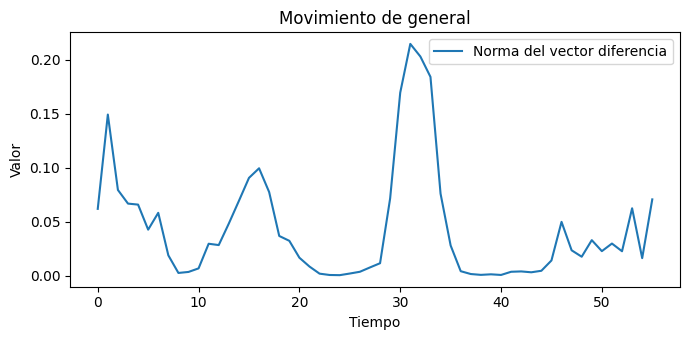
\includegraphics[align=t,width=0.9\linewidth, height=0.9\linewidth]{Graphics/aborto_global_movediff_original_nu.png}
		\caption{Gráfica de movimiento general del token ``aborto''}
		\label{f:general_movediff_aborto}
	\end{subfigure}
	\caption{Gráficas de movimiento por manos y general de los tokens ``amar'' y ``aborto''.}
	\label{f:movediff_aborto_amar}
\end{figure}


Resolver todos los problemas planteados anteriormente son fundamentales para la correcta generación de señas, puesto que, en caso de fallarse en solucionarse alguno de los problemas el resultado pudiera afectar negativamente la fluidez percibida por los usuarios, así como generar distorsiones durante la reproducción.
%%%%%%%%%%%%%%%%%%%%%%%
% POSIBLEMENTE PARA RECOMENDACIONES
